\documentclass[12pt]{extreport} % Schriftgröße: 8pt, 9pt, 10pt, 11pt, 12pt, 14pt, 17pt oder 20pt


%% Packages
\usepackage{scrextend}
\usepackage{amssymb}
\usepackage{amsthm}
\usepackage{booktabs}
\usepackage{chngcntr}
\usepackage{cmap}
\usepackage{color}
\usepackage{enumerate}
\usepackage{float}
\usepackage{hyperref}
\usepackage{ulem}
\usepackage{lmodern}
\usepackage{makeidx}
\usepackage{mathtools}
\usepackage{xpatch}
\usepackage{pgfplots}
\pgfplotsset{compat=1.7}
\usetikzlibrary{calc}	
\usetikzlibrary{matrix}	

% Language Setup (Deutsch)
\usepackage[utf8]{inputenc} 
\usepackage[T1]{fontenc} 
\usepackage[ngerman]{babel}

\usepackage{csquotes}
% Options
\makeatletter%%  
  % Publisher definieren
  \newcommand\publishers[1]{\newcommand\@publishers{#1}} 
  % Enumerate im 1. Level: \alph für a), b), ...
  \renewcommand{\labelenumi}{\alph{enumi})} 
  % Enumerate im 2. Level: \roman für (i), (ii), ...
  \renewcommand{\labelenumii}{(\roman{enumii})}
  % Zeileneinrückung am Anfang des Absatzes
  \setlength{\parindent}{0pt} 
  % Für das Proof-Environment: 'Beweis:' anstatt 'Beweis.'
  \xpatchcmd{\proof}{\@addpunct{.}}{\@addpunct{:}}{}{} 
  % Nummerierung der Bilder, z.B.: Abbildung 4.1
  \@ifundefined{thechapter}{}{\def\thefigure{\thechapter.\arabic{figure}}} 
\makeatother%

% Meta Setup (Für Titelblatt und Metadaten im PDF)
\title{Globale Optimierung}
\author{Prof. Dr. Oliver Stein}
\date{Sommersemester 2017}
\publishers{Karlsruher Institut für Technologie}

%% Math. Definitionen
\newcommand{\C}{\mathbb{C}}
\newcommand{\N}{\mathbb{N}}
\newcommand{\Q}{\mathbb{Q}}
\newcommand{\R}{\mathbb{R}}
\newcommand{\Z}{\mathbb{Z}}
\renewcommand*{\qed}{\hfill\ensuremath{\square}}

\theoremstyle{named}
\newtheorem{unnamedtheorem}{Theorem} 
\theoremstyle{nnamed}
\newtheorem*{unnamedtheorem*}{Theorem} 

\theoremstyle{itshape}
\newtheorem*{satz}{Satz} 
\newtheorem*{definition}{Definition}
\newtheorem*{hilfssatz}{Hilfssatz}

\theoremstyle{normal}
\newtheorem*{anwendung}{Anwendung}
\newtheorem*{beispiel}{Beispiel}
\newtheorem*{bemerkung}{Bemerkung} 
\newtheorem*{bezeichnung}{Bezeichnung}
\newtheorem*{eigenschaft}{Eigenschaft}
\newtheorem*{erinnerung}{Erinnerung}
\newtheorem*{folgerung}{Folgerung}
\newtheorem*{korollar}{Korollar}
\newtheorem*{lemma}{Lemma}
\newtheorem*{motivation}{Motivation}
\newtheorem*{uebung}{Übung}
\newtheorem*{vereinbarung}{Vereinbarung}

\makeatletter%
\DeclareUnicodeCharacter{00A0}{ } \pgfplotsset{compat=1.7} \hypersetup{colorlinks,breaklinks, urlcolor=linkcolor, linkcolor=linkcolor, pdftitle=\@title, pdfauthor=\@author, pdfsubject=\@title, pdfcreator=\@publishers}
\DeclareOption*{\PassOptionsToClass{\CurrentOption}{report}} 
\ProcessOptions 
\def\baselinestretch{1.25} \setlength{\oddsidemargin}{0.125in} \setlength{\evensidemargin}{0.125in} \setlength{\topmargin}{0.5in} \setlength{\textwidth}{6.25in} \setlength{\textheight}{8in} \addtolength{\topmargin}{-\headheight} \addtolength{\topmargin}{-\headsep} \def\pulldownheader{ \addtolength{\topmargin}{\headheight} \addtolength{\topmargin}{\headsep} \addtolength{\textheight}{-\headheight} \addtolength{\textheight}{-\headsep} } \def\pullupfooter{ \addtolength{\textheight}{-\footskip} } \def\ps@headings{\let\@mkboth\markboth \def\@oddfoot{} \def\@evenfoot{} \def\@oddhead{\hbox {}\sl \rightmark \hfil \rm\thepage} \def\chaptermark##1{\markright {\uppercase{\ifnum \c@secnumdepth >\m@ne \@chapapp\ \thechapter. \ \fi ##1}}} \pulldownheader } \def\ps@myheadings{\let\@mkboth\@gobbletwo \def\@oddfoot{} \def\@evenfoot{} \def\sectionmark##1{} \def\subsectionmark##1{}  \def\@evenhead{\rm \thepage\hfil\sl\leftmark\hbox {}} \def\@oddhead{\hbox{}\sl\rightmark \hfil \rm\thepage} \pulldownheader }	\def\chapter{\cleardoublepage  \thispagestyle{plain} \global\@topnum\z@ \@afterindentfalse \secdef\@chapter\@schapter} 
\def\@makeschapterhead#1{ {\parindent \z@ \raggedright \normalfont \interlinepenalty\@M \Huge \bfseries  #1\par\nobreak \vskip 40\p@ }} \newcommand{\indexsection}{chapter} \patchcmd{\@makechapterhead}{\vspace*{50\p@}}{}{}{}\def\Xint#1{\mathchoice
    {\XXint\displaystyle\textstyle{#1}} {\XXint\textstyle\scriptstyle{#1}} {\XXint\scriptstyle\scriptscriptstyle{#1}} {\XXint\scriptscriptstyle\scriptscriptstyle{#1}} \!\int} \def\XXint#1#2#3{{\setbox0=\hbox{$#1{#2#3}{\int}$} \vcenter{\hbox{$#2#3$}}\kern-.5\wd0}} \def\dashint{\Xint-} \def\Yint#1{\mathchoice {\YYint\displaystyle\textstyle{#1}} {\YYYint\textstyle\scriptscriptstyle{#1}} {}{} \!\int} \def\YYint#1#2#3{{\setbox0=\hbox{$#1{#2#3}{\int}$} \lower1ex\hbox{$#2#3$}\kern-.46\wd0}} \def\YYYint#1#2#3{{\setbox0=\hbox{$#1{#2#3}{\int}$}  \lower0.35ex\hbox{$#2#3$}\kern-.48\wd0}} \def\lowdashint{\Yint-} \def\Zint#1{\mathchoice {\ZZint\displaystyle\textstyle{#1}}{\ZZZint\textstyle\scriptscriptstyle{#1}} {}{} \!\int} \def\ZZint#1#2#3{{\setbox0=\hbox{$#1{#2#3}{\int}$}\raise1.15ex\hbox{$#2#3$}\kern-.57\wd0}} \def\ZZZint#1#2#3{{\setbox0=\hbox{$#1{#2#3}{\int}$} \raise0.85ex\hbox{$#2#3$}\kern-.53\wd0}} \def\highdashint{\Zint-} \DeclareRobustCommand*{\onlyattoc}[1]{} \newcommand*{\activateonlyattoc}{ \DeclareRobustCommand*{\onlyattoc}[1]{##1} } \AtBeginDocument{\addtocontents{toc} {\protect\activateonlyattoc}} 
	% Titlepage
	\def\maketitle{ \begin{titlepage} 
			~\vspace{3cm} 
		\begin{center} {\Huge \@title} \end{center} 
	 		\vspace*{1cm} 
	 	\begin{center} {\large \@author} \end{center} 
	 	\vspace*{-0.5cm}
	 	\begin{center} \@date \end{center} 
	 		\vspace*{7cm} 
	 	\begin{center} \@publishers \end{center} 
	 		\vfill 
	\end{titlepage} }
\makeatother%


% Create Index
\makeindex 

\begin{document}

\thispagestyle{empty}

\pagenumbering{Alph}
\begin{titlepage}
	\maketitle
	\thispagestyle{empty}
\end{titlepage}

% Skript - Anfang 			
\pagenumbering{arabic}

% todo online fragen

\chapter{Einführungen}

\section{Grundbegriffe}

Zwei grundlegende Begriffe in der Optimierung sind der \textbf{optimale Punkt} und der \textbf{optimale Wert}. Als Beispiel kann man fragen, wer in einer Gruppe von Personen die meisten Münzen bei sich trägt. Der optimale Wert ist die gefundene größtmögliche Anzahl von Münzen. Er ist eindeutig bestimmt. Im Gegensatz dazu können durchaus mehrere Personen diese Anzahl von Münzen bei sich tragen. Demnach ist der Punkt (hier: die Person), an dem der optimale Wert angenommen wird, nicht notwendigerweise eindeutig. Dies gilt analog bei jedem Optimierungsproblem.

\begin{beispiel}[Projektion auf eine Menge] ~\\
Sei $M \subseteq \R^n$ und $z \in \R^n$
$$ P_M: \quad \min_{x \in \R^n} \| x - z \|_2 \text{ s.t. } x \in M. $$
Nach Satz 1.2.10 ist dieses Projektionsproblem für jede nicht-leere und kompakte Menge $M \subseteq \R^n$ lösbar, denn $\| \cdot \|_2$ ist eine stetige Funktion. ~\\

\textit{Beachte: Projektion unter euklidischer Norm = orthogonale Projektion} ~\\

Falls $M$ eine Hyperebene ist, lässt sich das Problem $P_M$ explizit lösen. Dazu sei 
$$ M = \left\{ x \in \R^n \colon a^T x = b \right\}, $$
d.h. $M$ sei durch eine lineare Gleichung beschrieben. Dann wird das Optimierungsproblem $P$ zu
$$ P_M\colon \min_{x \in \R^n} \| x - z \|_2 \text{ s.t. } a^Tx = b $$
damit ist der eindeutige optimale Punkt $\overline{x}$ und der dazugehörige optimale Wert $v$ gegeben durch
$$ \overline{x} = z - \frac{a^T z - b}{a^T a} \cdot a, ~ v = \left| \frac{a^T z - b}{a^T a} \cdot a \right|_2 = \frac{\left| a^T z - b \right|}{\| a \|_2}$$
\end{beispiel}


\begin{definition}[Minimalpunkte und Minimalwerte] ~\\
	Gegeben sei eine Menge von zulässigen Punkte $M \subseteq \R$ und eine Zielfunktion $f \colon M \rightarrow \R$.
	\begin{enumerate}
		\item $\overline{x} \in M$ heißt \textbf{lokaler Minimalpunkt} von $f$ auf $M$, falls eine Umgebung $U$ von $\overline{x}$  existiert mit
			$$ \forall x \in U \cap M: \quad f(x) \geq f(\overline{x}). $$
		\item $\overline{x} \in M$ heißt \textbf{globaler Minimalpunkt} von $f$ auf $M$, falls man in a) $U = \R^n$ wählen kann.
		\item Ein lokaler oder globaler Minimalpunkt heißt \textbf{strikt}, falls in a) bzw. b) für $x \neq \overline{x}$ sogar die strikte Ungleichung \enquote{$>$} gilt.
		\item Zu jedem globalen Minimalpunkt $\overline{x}$ heißt $f(\overline{x})$ ($= v = \min_{x \in M} f(x)$) \textbf{globaler}, und zu jedem lokalen Minimalpunkt $\overline{x}$ heißt $f(\overline{x})$ \textbf{lokaler Minimalwert}.
	\end{enumerate}
	Strikte globale Minimalpunkte sind eindeutig, und strikte lokale Minimalpunkte sind lokal eindeutig.
\end{definition}

\begin{beispiel}[1.1.5, 1.2.26, 1.2.31 Zentrum einer Punktewolke] ~\\
	Gegeben seien Punkte $x^1, x^2, \dotsc, x^m \in \R^n$. Gesucht ist ein Punkt $z \in \R^n$ \enquote{im Zentrum der Punkte}. Benutzt man die 2-Norm so führt dies auf das Optimierungsproblem
		$$ P: \quad \min_{z \in \R^n} \left\| \left( \| z - x^2 \|_2, \dotsc \| z - x^m \|_2 \right)^T \right\|_2, $$
	ohne Nebenbedingungen. Als Optimalpunkt berechnet man das arithmetische Mittel der Punkte
	$$ \overline{z} = \frac{1}{m} \sum_{i=1}^m x^i. $$
	Ein Problem dieses Ansatzes besteht darin, dass Ausreißer bei wachsender Punkteanzahl $m$ vernachlässigt werden. Eine Möglichkeit dieses Problem zum umgehen, könnte 
	$$ \| x \|_\infty = \max_{j=1, \dotsc, n} |x_j| $$ 
	als äußere Norm zu verwenden. ~\\
	
	Dieses Problem ist koerziv, denn es gilt
	$$ f(z) = \sqrt{\sum_{i=1}^m \| z - x^i \|_2^2} \geq \sqrt{\| z - x^1 \|_2^2} = \| z - x^1 \| \geq \left| \| z \| - \| x^1 \|_2 \right| \xrightarrow[\| z\|\rightarrow \infty]{} +\infty $$
	Somit ist dieses Beispiel nach 1.2.26 und Korollar 1.2.30 lösbar.
\end{beispiel}

\begin{definition}[Epigraph]
	Für $M \subseteq \R^n$ und $f \colon M \rightarrow \R$ heißt die Menge
	$$ \operatorname{epi}(f, M) = \big\{ (x, \alpha) \in M \times \R ~|~ f(x) \leq \alpha \big\} $$
	\textbf{Epigraph} von $f$ auf $M$. Der Epigraph besteht aus dem Graphen von $f$ auf $M$ sowie allen darüber liegenden Punkten.
\end{definition}

Die Suche nach einem Minimalpunkt von $f$ auf $m$ ist äquivalent zur Suche nach einem $(x, \alpha)$ mit minimaler $\alpha$-Komponente auf dem Epigraphen von $f$ (vgl. Übung 1.3.7). % todo Uebung

\begin{definition}[Epigraph-Umformulierung]
	Das Problem 
		$$ P: \quad \min_x f(x) \text{ s.t. } x \in M $$
	ist in diesem Sinne also äquivalent zu
		$$ P_{epi}: \quad \min_{(x, \alpha)} \alpha \text{ s.t. } f(x) \leq \alpha, ~x \in M. $$
\end{definition}

\begin{beispiel}[Epigraph-Umformulierung der Punktewolke] ~\\
	Im vorliegenden Fall des Zentrums einer Punktwolke mit Maximumsnorm als äußerer Norm gilt
		$$ P: \quad \min_{z \in \R^n} \left\| \left( \| z - x^2 \|_2, \dotsc \| z - x^m \|_2 \right)^T \right\|_2, $$
	also $M = \R^n$ und 
		$$ f(z) = \max_{i=1, \dotsc, m} \| z - x^i \|_2. $$
	Die Epigraph-Umformulierung lautet dann
		$$ P_{epi}: \quad \min_{(z, \alpha)} \alpha \text{ s.t. } f(z) \leq \alpha, $$
	wobei die Nebenbedingung von $P_{epi}$ ausgeschrieben lautet:
	$$ \max_{i=1, \dotsc, m} \| z - x^i \|_2 \leq \alpha; $$
	bzw. das Maximum ausnutzend:
	$$ P_{epi}: \quad \min_{(z, \alpha)} \alpha \text{ s.t. } \| z - x^i \|_2 \leq \alpha, ~ i = 1, \dotsc, m $$
	d.h. man sucht einen Kreis mit Mittelpunkt $z$ und minimalem Radius $\alpha$ zu finden, der alle Punkte $x^1, \dotsc, x^m$ enthält.
\end{beispiel}

\begin{beispiel}[1.1.6, 1.2.27, Clusteranalyse]
	Anstatt wie bei der Punktewolke nur nach einem Mittelpunkt zu suchen, gehen wir nun von $k$ Zentren aus. Das Problem ergibt sich dann zu
	$$ P: \quad \min_{z^1, \dotsc, z^k \in \R^n} \left\| \left( \min_{\ell = 1, \dotsc, k} \| z^{\ell} - x^1 \|, \dotsc, \min_{\ell = 1, \dotsc, k} \| z^\ell - x^m \| \right)^T \right\| $$ 
	Als äußere Norm benutzt man häufig die $\ell_1$-Norm, d.h.
	$$ P_1: \quad \min_{z^1, \dotsc, z^k \in \R^n} \sum_{i=1}^{m} \min_{\ell = 1, \dotsc, k} \| z^\ell - x^i \| $$
	oder auch die $\ell_\infty$-Norm mit
	$$ P_\infty: \quad \min_{z^1, \dotsc, z^k \in \R^n} \max_{i=1, \dotsc, m} \min_{\ell = 1, \dotsc, k} \| z^\ell - x^i \|. $$	
	Beachte: der Vektor der Entscheidungsvariable im Problem hat in jedem Fall die Dimension $n \cdot k$, so dass in praktisch relevanten Anwendungen häufig hochdimensionale Probleme auftreten. Dieses Problem ist nicht koerziv.
\end{beispiel}

\newpage

\section{Lösbarkeit}

\begin{definition}[Infimum]
	Wir bezeichnen mit $\alpha \in \R$ die \textbf{untere Schranke} für $f$ auf $M$, falls
	$$ \forall x \in M: \quad \alpha \leq f(x) $$
	gilt. Das \textbf{Infimum} von $f$ auf $M$ ist die größte untere Schranke von $f$ auf $M$, es gilt also $v = \inf_{x \in M} f(x)$ falls
	\begin{itemize}
		\item $\forall x \in M$: $v \leq f(x)$ (d.h. $v$ ist selbst untere Schranke) und
		\item für alle unteren Schranken $\alpha$ von $f$ auf $M$ als kleinste obere Schranke definiert.
	\end{itemize}
	Analog wird das \textbf{Supremum} $\sup_{x \in M} f(x)$ von $f$ auf $M$ als kleinste obere Schranke definiert. ~\\
	
	Falls $f$ auf $M$ nicht nach unten beschränkt ist, setzt man formal
	$$ \inf_{x \in M} f(x) = - \infty, $$
	und für das Infimum über die leere Menge definiert man formal
	$$ \inf_{x \in \emptyset} f(x) = +\infty. $$
\end{definition}

\begin{definition}[1.2.3, Lösbarkeit]
	Das Minimierungsproblem $P$ heißt \textbf{lösbar}, falls ein $\overline{x} \in M$ mit $\inf_{x \in M} f(x) = f(\overline{x})$ existiert. ~\\
	
	Um anzudeuten, dass das Infimum angenommen wird, schreiben wir $\min_{x \in M} f(x)$ anstelle von $\inf_{x \in M} f(x)$.
\end{definition}

\begin{satz}[1.2.5]
	Das Minimierungsproblem $P$ ist genau dann lösbar, wenn es einen globalen Minimalpunkt besitzt.
\end{satz}

\newpage

\section{Arten von Unlösbarkeit}

\begin{definition}[1.2.6]
	Wir bezeichnen mit $\operatorname{pr}(z, M)$ die Menge der \textbf{orthogonalen Projektionen} eines Punktes $z \in \R^n$ auf $M \subseteq \R^n$ und mit
	$$ \operatorname{pr}(Z, M) = \big\{ \operatorname{pr}(z, M) ~|~ z \in M \big\} $$
	die orthogonale Projektion einer Menge $Z \subseteq \R^n$ auf $M$.
\end{definition}

\begin{definition}[1.2.7, Parallelprojektion]
	Für $Z \subseteq \R^n = R^k \times R^\ell$ heißt
	$$ \operatorname{pr}_a(Z) = \big\{ a \in \R^k ~|~\exists b \in \R^\ell \colon (a, b) \in Z \big\}. $$
	\textbf{Parallelprojektion} von $Z$ in die Menge $\R^k$.
\end{definition}

\begin{folgerung}[Parallelprojektion der Epigraphen]
	Die Parallelprojektion von $\operatorname{epi}(f, M)$ auf den \enquote{$\alpha$-Raum} $\R$ lautet also
	$$ \operatorname{pr}_\alpha \operatorname{epi}(f, M) = \big\{ \alpha \in \R ~|~\exists x \in M: f(x) \leq \alpha \big\} $$
\end{folgerung}

\begin{satz}[1.2.8]
	Für jedes Optimierungsproblem $P$ hat die Menge $\operatorname{pr}_{\alpha} \operatorname{epi}(f, M)$ genau eine der vier Gestalten
	\begin{enumerate}
		\item $\operatorname{pr}_{\alpha} \operatorname{epi}(f, M) = \emptyset$
		\item $\operatorname{pr}_{\alpha} \operatorname{epi}(f, M) = \R$
		\item $\operatorname{pr}_{\alpha} \operatorname{epi}(f, M) = (v, +\infty)$ mit $v \in \R$
		\item $\operatorname{pr}_{\alpha} \operatorname{epi}(f, M) = [v, +\infty)$ mit $v \in \R$
	\end{enumerate}
	Ferner ist der Fall a) zu $M =\emptyset$ % todo missing
\end{satz}

\begin{beispiel}[Distanz eines Punktes von einer Menge]
	Für eine Menge $M \subseteq \R^n$ und einen Punkt $z \in \R^n$ heißt
	$$ \operatorname{dist}(z, M) \coloneqq \inf_{x \in M} \| x - z \|_2 $$	
	Distanz von $z$ zu $M$. Wegen der Nichtnegativität der Norm ist Unlösbarkeit wegen Unbeschränktheit für dieses Problem nicht möglich. Ferner gilt 
	$$ \operatorname{dist}(z, \emptyset) = +\infty \text{ für jedes } z \in \R^n. $$
	Beachte: die fehlende Abgeschlossenheit von $M$ führt hier zu Unlösbarkeit.
\end{beispiel}

\newpage

\section{Der Satz von Weierstraß}

Eine Minimalvoraussetzung für die Lösbarkeit ist offensichtlich die Konsistenz von $M$, also $M \neq \emptyset$.

\begin{satz}[1.2.10, Satz von Weierstraß]
	Die Menge $M \subseteq \R^n$ sei nicht-leer und kompakt, und die Funktion $f \colon M \rightarrow \R$ sei stetig. Dann besitzt $f$ auf $M$ einen globalen Minimalpunkt und einen globalen Maximalpunkt. ~\\
	
	Beachte: außer der Konsistenz von $M$ keine dieser Bedingungen auch notwendig für Lösbarkeit ist.	Dass die Bedingungen stärker als nötig sind, sieht man alleine schon daran, auch die Existenz eines globalen Maximalpunkts garantiert wird.
\end{satz}

\begin{definition}[Untere Niveaumenge]
	Für $M \subseteq \R^n$, $f \colon M \rightarrow \R$ und $\alpha \in \overline{\R}$ heißt
	$$ \operatorname{lev}_{\leq}^{\alpha}(f, \R^n) = \big\{ x \in M ~|~f(x) \leq \alpha \big\} $$
	\textbf{untere Niveaumenge} von $f$ auf $M$ zum Niveau $\alpha$. Im Falle $M = \R^n$ schreiben wir auch kurz
	$$ f_{\leq}^\alpha \coloneqq \operatorname{lev}_{\leq}^{\alpha}(f, \R^n) = \big\{ x \in \R^n ~|~ f(x) \leq \alpha \big\} $$
	Für jede reellwertige Funktion $f$ gilt $\operatorname{lev}_{\leq}^{+\infty}(f, M) = M$ und $\operatorname{lev}_{\leq}^{-\infty}(f, M) = \emptyset$. In der Analysis wird gezeigt, dass für stetiges $f$ die Mengen $f_{\leq}^{\alpha}$ für alle $\alpha \in \R$ abgeschlossen sind. ~\\
	
	Beachte: $\operatorname{lev}_{\leq}^{\alpha}(f, \R^n) \neq \operatorname{epi}(f, M)$, bzw.
	$$ \big\{ x \in M ~|~f(x) \leq \alpha \big\} \neq \big\{ (x, \alpha) \in M \times \R ~|~f(x) \leq \alpha \big\} $$ 
\end{definition}

\begin{definition}[Menge der Minimalpunkte]
	Wir führen die Menge der globalen Minimalpunkte
	$$ S = \big\{ \overline{x} \in M ~|~ \forall x \in M : f(x) \geq f(\overline{x}) \big\} $$
	von $P$ ein. Die Lösbarkeit von $P$ ist dann zu $S \neq \emptyset$ äquivalent.
\end{definition}

\begin{lemma}[1.2.13]
	Es sei $v = \inf_{x \in M} f(x)$. Dann gilt $S = \operatorname{lev}_{\leq}^{v}(f, M)$.	
\end{lemma}

\begin{lemma}[1.2.15]
	Für ein $\alpha \in \R$ sei $\operatorname{lev}_{\leq}^{\alpha}(f, M) \neq \emptyset$. Dann gilt $S \subseteq \operatorname{lev}_{\leq}^{\alpha}(f, M)$.
\end{lemma}

\begin{satz}[1.2.16, Verschärfter Satz von Weierstraß]
	Für eine Menge $M \subseteq \R^n$ sei $f \colon M \rightarrow \R$ stetig, und mit einem $\alpha \in \R$ sei $\operatorname{lev}^{\alpha}_{\leq}(f, M)$ nicht-leer und kompakt. Dann ist auch $S$ nicht-leer und kompakt.	
\end{satz}

\begin{beispiel}
	Betrachtet werde das Problem	 ~\\
	
	\begin{figure*}[h!] \centering
		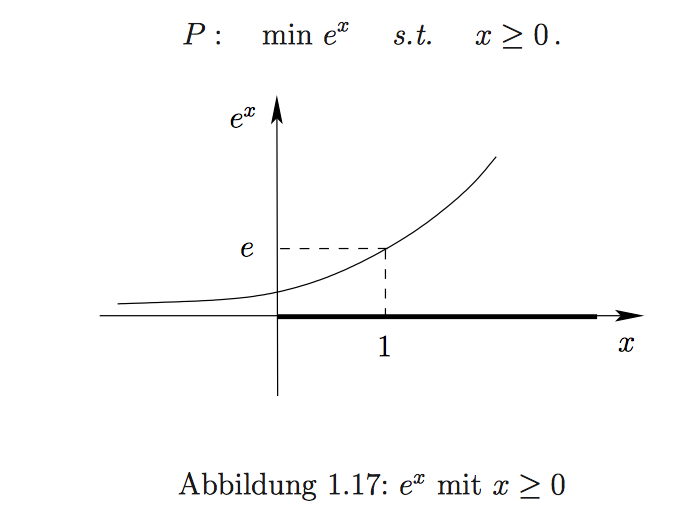
\includegraphics[scale=0.5]{img/ks-i}
	\end{figure*}
	~\\
	Hier ist $M = \big\{ x \in \R ~|~x \geq 0 \big\}$ unbeschränkt, der Satz von Weierstraß (Satz 1.2.10) also nicht anwendbar. Aber beispielsweise mit $\alpha = e$ ist
	$$ \operatorname{lev}_{\leq}^{e}(f, M) = \big\{ x \in M ~|~e^x \leq e \big\} = \big\{ x \geq 0 ~|~x \leq 1 \big\} = [0, 1] $$
	nicht-leer und kompakt. Folglich ist der Verschärften Satz von Weierstraß (Satz 1.2.16) anwendbar und $P$ daher lösbar.
\end{beispiel}

\begin{korollar}[1.2.19, Verschärfter Satz von Weierstraß für unrestringierte Probleme]
Sei $f \colon \R^n \rightarrow \R$ stetig und mit einem $\alpha \in \R$ sei $f_{\leq}^{\alpha}$ nicht-leer und kompakt. Dann ist auch $S$ nicht-leer und kompakt.	
\end{korollar}

\begin{definition}[1.2.23, Koerzivität bei $\infty$]
	Gegeben sei eine Funktion $f \colon M \rightarrow \R$ mit $M \subseteq \R^n$. Falls für alle Folgen $(x^\nu) \subseteq M$ mit $\lim_\nu \| x^\nu \| \rightarrow +\infty$ auch
	$$ \lim_\nu f(x^\nu) = +\infty $$
	gilt, dann heißt $f$ koerziv bei $\infty$ auf $M$. Falls $M$ abgeschlossen ist, heißt $f$ kurz koerziv auf $M$.
\end{definition}

\begin{beispiel}[1.2.28, Beispiel]
	Auf kompakten Mengen $M$ ist jede Funktion $f$ trivialerweise koerziv.
\end{beispiel}
 
\begin{lemma}[1.2.29]
	Die Funktion $f \colon M \rightarrow \R$ sei koerziv bei $\infty$ auf der Menge $M \subseteq \R^n$. Dann sind die Mengen $\operatorname{lev}_{\leq}^{\alpha}(f, M)$ für jedes Niveau $\alpha \in \R$ beschränkt.	
\end{lemma}

\begin{korollar}[1.2.30]
	Es sei $M$ nicht-leer und abgeschlossen und $f \colon M \rightarrow \R$ sei stetig und koerziv auf $M$. Dann ist $S$ nicht-leer und kompakt.
\end{korollar}

\begin{bemerkung}[1.2.35]
	Auf der abgeschlossenen Menge $X \subseteq \R^n$ seien die Funktionen $f, g_i$, $i \in I$, stetig, die Menge 
	$$ \big\{ x \in X ~|~g_i(x) \leq0, i \in I \big\} $$
	 sei nicht-leer, und mindestens eine der Funktionen $f, g_i$, $i \in I$, sei koerziv auf $X$. Zeigen Sie, dass die Menge $S$ der Optimalpunkte von $f$ auf $M$ dann nicht-leer und kompakt ist.
\end{bemerkung}


\begin{definition}[1.2.37, Koerzivität]
	Gegeben seien eine (nicht notwendigerweise abgeschlossene) Menge $M \subseteq \R^n$ und eine Funktion $f \colon M \rightarrow \R$. Falls für alle Folgen $(x^\nu) \subseteq M$ mit $\lim_\nu \| x^\nu \| \rightarrow \infty$ und alle konvergenten Folgen $(x^\nu) \subseteq M$ mit $\lim_\nu x^\nu \notin M$ die Bedingung 
	$$ \lim_\nu f(x^\nu) = +\infty $$
	gilt, dann heißt $f$ \textbf{koerziv} auf $M$.
\end{definition}

\begin{beispiel}[1.2.36, 1.2.38]
	Gegeben seien $N$ Beobachtungen $\hat{x}_1, \dotsc, \hat{x}_N \geq 0$ mit $\overline{x} = \frac{1}{N} \sum_{i=1}^{N} \hat{x}_i > 0$, die als Realisierungen stochastisch unabhängiger und mit Parameter $\lambda > 0$ exponentialverteilerter Zufallsvariablen $X_1, \dotsc, X_N$ aufgefasst werden. Gesucht ist der Parameter $\lambda$, der zu den Beobachtungen \enquote{am besten passt}. Dazu kann man mit Hilfe der Dichtefunktionen der einzelnen $X_i$,
	$$ f(\lambda x_i) = \begin{cases}
		\lambda e^{-\lambda x_i}, & x_i \geq 0 \\ 0, & x_i < 0,
	\end{cases} $$
	zunächst die gemeinsame Dichte aller Zufallsvariabelen
	$$ L(\lambda, x) = \Pi_{i=1}^{N} f(\lambda, x_i) $$
	betrachten. Der Maximum-Likelihood-Schätzer bestimmt dann $\lambda$ als optimalen Punkt des Problems
	$$ ML: \quad \max_{\lambda} L(\lambda, \tilde{x}) \text{ s.t. } \lambda > 0. $$
	Die zulässige Menge $M = (0, \infty)$ dieses Problems ist offensichtlich nicht abgeschlossen. Es sit auch sinnlos, den Parameterwert $\lambda = 0$ künstlich hinzuzufügen, da $f(0, x)$ keine Wahrscheinlichkeitsdichte ist. ~\\
	
	Wir werden im Folgendens sehen, wie die Lösbarkeit dieses Problems trotzdem garantiert werden und später auch einen globalen Maximalpunkt bestimmen. Dazu berechnen wir zunächst
	$$ L(\lambda, \hat{x}) = \Pi_{i=1}^{N} \lambda e^{-\lambda \hat{x}_i} = \lambda^N e^{-\lambda N \overline{x}}, \ell(\lambda, \hat{x}) \coloneqq \log(L(\lambda, \hat{x})) = N \log(\lambda) - \lambda N \overline{x} $$
	Da die Funktion $\log$ streng monoton wachsend auf dem Bildbereich $(0, \infty)$ von $L$ ist, kann man Hilfe von Übung 1.3.5 zeigen, dass das Problem
	$$ ML_{log}: \quad \max_\lambda \ell(\lambda, \hat{x}) \text{ s.t. } \lambda > 0 $$
	dieselben Optimalpunkte wie $ML$ besitzt. Schließlich streichen wir mittels Übung 1.3.1a) die Konstante $N > 0$ aus der Zeilfunktion und gehen zum äquivalenten Minimierungsproblem
	$$ P_{LM}: \quad \min_\lambda \lambda \overline{x} - \log(\lambda) \text{ s.t. } \lambda > 0 $$
	über.
	
% todo  kann man Hilfe von Übung 1.3.5 zeigen, dass das Problem ... Schließlich streichen wir mittels Übung 1.3.1a) die Konstante N

	Für $\overline{x} > =$ ist die Zielfunktion $f(\lambda) = \lambda \overline{x} - \log(\lambda)$ des Problems $P_{ML}$ koerziv auf $M = (0, \infty)$. Wir merken an, dass nur die Log-Likelihood-Funktion $\ell$ zu Koerzivität führt, die Likelihood-Funktion $L$ selbst aber nicht. ~\\
	
	Das Problem $P_{ML}$ und damit auch das Problem $ML$ sind nach Korollar 1.2.40 lösbar.
\end{beispiel}

\begin{lemma}[1.2.39]
	Die Funktion $f \colon M \rightarrow \R$ sei stetig und koerziv auf der Menge $M \subseteq \R^n$. Dann sind die Mengen $\operatorname{lev}_{\leq}^{\alpha}(f, M)$ für jedes Niveau $\alpha \in \R$ kompakt.
\end{lemma}

\begin{korollar}[1.2.40]
	Es sei $M$ nicht-leer, und $f \colon M \rightarrow \R$ seis tetig und koerziv auf $M$. Dann ist $S$ nicht-leer und kompakt.
\end{korollar}

\begin{bemerkung}[Rechenregeln] ~\
	\begin{itemize}
		\item Skalare und Vielfache (1.3.1) $\alpha \geq 0: ~ \min_{x \in M} \left( \alpha f(x) + \beta \right) = \alpha \left( \min_{x \in M} f(x) \right) + \beta$,
			$$ \alpha < 0:  \min_{x \in M} \left( \alpha f(x) + \beta \right) = \alpha \left( \max_{x \in M } f(x) \right) + \beta, \quad \min_{x \in M} \left( f(x) + g(x) \right) \geq \min_{x \in M} f(x) + \min_{x \in M} g(x) $$
		\item $\min_{x \in X} \max_{y \in Y} f(x, y) \geq \max_{y \in Y} \min_{x \in X} f(x, y)$
		 \item Monotone Transformation (1.35) $M \subseteq \R^n$, $f \colon M \rightarrow Y$ und $\psi \colon Y \rightarrow \R$ eine streng monotone wachsende Funktion. Dann gilt
		 	$$ \min_{x \in M} \psi(f(x)) = \psi (\min_{x \in M} f(x)) $$
		 \item Projektionsumformulierung (1.3.6): folgende Probleme sind äquivalent
		 	$$ P: \quad \min_{(x,y) \in \R^n \times \R^m} f(x) \text{ s.t. } (x, y) \in M $$
		 	und
		 	$$ P_{proj}: \quad \min_{x \in \R^n} f(x) \text{ s.t. } x \in \operatorname{pr}_x M $$
		 \item Monotones Funktional (1.3.8): wir nennen $F \colon \R^k \rightarrow \R$ monoton, falls $x \leq y \Rightarrow F(x) \leq F(y)$.
	\end{itemize}
\end{bemerkung}

\begin{bemerkung}[1.3.7, Epigraph Umformulierung]
	Gegeben seien $M \subseteq \R^n$ und eine Funktion $f \colon M \rightarrow \R$. Dann sind die folgenden Probleme äquivalent:
	$$ P: \quad \min_{x \in \R^n} f(x) \text{ s.t. } x \in M $$
	und 
		$$ P_{epi}: \quad \min_{(x, \alpha) \in \R^n \times \R} \alpha \text{ s.t. } f(x) \leq \alpha, x\in M $$
\end{bemerkung}

\begin{bemerkung}[1.3.9, Verallgemeinerte Epigraph Umformulierung]
	Gegeben seien $X \subseteq \R^n$, Funktionen $f \colon X \rightarrow \R^k$ und $g \colon X \rightarrow R^\ell$ sowie monotone Funtkionen $F \colon \R^k \rightarrow \R$ und $G \colon \R^\ell \rightarrow \R$. Dann sind die folgenden Probleme äquivalent:
	$$ P: \quad \min_{x \in \R^n} F(f(x)) \text{ s.t. }~ G(g(x)) \leq 0, x \in M $$
	und 
		$$ P_{epi}: \quad \min_{(x, \alpha, \beta) \in \R^n \times \R^k \times \R^\ell} F(\alpha) ~\text{ s.t. }~ G(\beta) \leq 0,  f(x) \leq \alpha, ~ g(x) \leq \beta, ~ x\in M $$
\end{bemerkung}

\chapter{Konvexe Optimierungsprobleme}

\section{Konvexität}

\begin{definition}[2.1.1, Konvexe Mengen und Funktionen] ~\
	\begin{enumerate}
		\item Eine Menge $M \subseteq \R^n$ heißt konvex, falls $\forall x, y \in M, \lambda \in (0, 1)$: $(1 - \lambda) x + \lambda y \in M$ gilt. Konvexe Mengen brauchen weder beschränkt noch abgeschlossen zu sein.
		\item Für eine konvexe Menge $M \subseteq \R^n$ heißt eine Funktion $f \colon M \rightarrow \R$ konvex, falls
			$$ \forall x, y \in M, \lambda \in (0, 1): \quad f( (1-\lambda)x + \lambda y) \leq (1- \lambda) f(x) + \lambda f(y) $$
			d.h. der Funktionsgraph von $f$ verläuft unter jeder seiner Sekanten.
		\item Für eine konvexe Menge $M \subseteq \R^n$ heißt eine Funktion $f \colon M \rightarrow \R$ strikt konvex, falls in b) für $x \ne y$ sogar die strikte Ungleichung gilt.
		\item Für eine konvexe Menge $M \subseteq \R^n$ heißt eine Funktion $f \colon M \rightarrow \R$ gleichmäßig konvex (auf $M$), falls mit einer Konstanten $c > 0$ die Funktion $f(x) - \frac{c}{2} \| x \|_2^2$ konvex auf $M$ ist.
		\item Für eine konvexe Menge $M \subseteq \R^n$ heißt eine Funktion $f \colon M \rightarrow \R$ konkav, strikt konkav oder gleichmäßig konkav (auf $M$) falls $-f$ konvex, strikt konvex bzw. gleichmäßig konvex auf $M$ ist.
	\end{enumerate}
\end{definition}

\begin{uebung}[2.1.2] % todo Uebung
	Auf einer konvexen Menge $M \subseteq \R^n$ ist die Funktion $f \colon M \rightarrow \R$ genau dann konvex, wenn die Mengen $\operatorname{epi}(f, M)$ konvex ist.	
\end{uebung}

\begin{definition}[2.1.3, Konvexes Optimierungsproblem]
	Das Optimierungsproblem
	$$ P: \quad \min f(x) \text{ s.t. } x \in M $$
	heißt \textbf{konvex}, falls $M$ und $f \colon M \rightarrow \R$ konvex sind. ~\\
	
	Da $M = \R^n$ eine konvexe Menge ist, sind unrestringierte Probleme genau dann konvex, wenn $f$ konvex auf $\R^n$ ist.
\end{definition}

\begin{satz}[2.1.4]
	$P$ sei konvex. Dann ist jeder lokale Minimalpunkt von $P$ auch globaler Minimalpunkt von $P$. ~\\
	
	Der Grund für diesen Effekt liegt darin, dass Konvexität eine globale Voraussetzung an $P$ ist.	
\end{satz}

\begin{uebung}[2.1.5] % todo Uebung
	Die Menge $M \subseteq \R^n$ und die Funktion $f \colon M \rightarrow \R$ seien konvex. Dann ist $\operatorname{lev}_{\leq}^{\alpha}(f, M)$ für jedes $\alpha \in \overline{\R}$ konvex. Die Umkehrung dieser Aussage ist falsch.	
\end{uebung}

\begin{uebung}[2.1.6]
	Der Schnitt beliebig vieler konvexer Mengen ist konvex.	
\end{uebung}

\begin{korollar}[2.1.8]
	Mit beliebigen Indexmengen $I, J$ seien die Funktionen $g_i \colon \R^n \rightarrow \R$, $i \in I$, konvex, und die Funktionen $h_j \colon \R^n \rightarrow \R$, $j \in J$, linear. Dann ist die Menge
	$$ M = \big\{ x \in \R^n ~|~g_i(x) \leq 0, i \in I, h_j(x) = 0, j \in J \big\} $$
	konvex.
\end{korollar}

\begin{beispiel}[2.1.9]
	Falls $f, g_i$ auf $\R^n$ konvex und $h_j$ lineare Funktionen sind, dann ist
	$$ P: \quad \min f(x) \text{ s.t. } g_i(x) \leq 0, ~ i \in I,~h_j(x) = 0, ~j \in J $$	
	ein konvexes Optimierungsproblem.
\end{beispiel}

\begin{beispiel}[2.1.10]
	Mit $c \in \R^n$, $b \in \R^m$ und einer $(m, n)$-Matrix $A = (a_1^T, \dotsc, a_m^T)^T$ mit $a_i \in \R^n$ ist
	$$ P: \quad \min c^T x \text{ s.t. } Ax \leq b $$
	ein lineares Optimierungsproblem (die Ungleichungsnebenbedingungen können sowohl eine Nichtnegativitätsbedingung $x \geq 0$ enthalten als auch Gleichungen modellieren). ~\\
	
	$P$ ist auch ein konvexes Optimierungsproblem, denn mit den Setzungen $f(x) = c^T x$, und $g_i(x) = a_i^T x - b_i$ sind $f, g_i \colon \R^n \rightarrow \R$ linear und damit konvex auf $\R^n$. ~\\
	
	Zum Beispiel setzt man für das lineare Optimierungsproblem
	$$ \min x_1 + x_2 \text{ s.t. } x \geq 0 $$
	$f(x) = x_1 + x_2$, $g_1(x) = - x_1$ und $g_2(x) = -x_2$.
\end{beispiel}

\section{$C^1$-Charakterisierung}

\begin{bemerkung}[Kettenregel] $D(f \circ g)(\overline{x}) = D f(g(\overline{x})) \cdot D g(\overline{x})$	
\end{bemerkung}

\begin{satz}[2.2.1, Linearisierung per Satz von Taylor im $\R^n$]
	Für eine nicht-leere, offene und konvexe Menge $U \subseteq \R^n$ sei die Funktion $f \colon \rightarrow \R$ differenzierbar an $x \in U$. Dann gilt für alle $y \in U$	
	$$ f(y) = f(x) + \langle \nabla f(x), y - x \rangle + o \left( \| y - x \| \right), $$
	wobei $o \left( \| y - x \| \right)$ einen Ausdruck der Form $w(y) \| y - x \|$ mit einer an $x$ stetigen Funktion $w$ mit $w(x) = 0$ bezeichnet.
\end{satz}

\begin{satz}[2.2.2., $C^1$-Charakterisierung von Konvexität]
	Auf einer konvexen Mengen $M \subseteq \R^n$ ist eine Funktion $f \in C^1(M, \R)$	 genau dann konvex, wenn folgendes gilt
	$$ \forall x, y \in M: \quad f(y) \geq f(x) + \langle \nabla f(x), y - x \rangle $$
	Die $C^1$-Charakterisierung besagt, dass eine $C^1$-Funktion genau dann konvex auf $M$ ist, wenn ihr Graph über jeder seiner Tangentialebenen verläuft.
\end{satz}

\section{Lösbarkeit}

Für die Lösbarkeit von $P$ ist Konvexität alleine kein wesentlicher Vorteil: sowohl $f_1(x) = (x - 5)^2$ als auch $f_2(x) = e^x$ sind sogar strikt konvex, aber nur $f_1$ besitzt einen globalen Minimalpunkt auf $\R$. Im Folgenden werden wir sehen, dass der entscheidende Vorteil von $f_1$ gegenüber $f_2$ die gleichmäßige Konvexität ist.

\begin{uebung}[2.3.1] % todo Uebung
	Für eine konvexe Menge $M \subseteq \R^nle$ sei $f \colon M \rightarrow \R$ gleichmäßig konvex. Dann ist $f$ auch strikt konvex auf $M$.	
\end{uebung}

\begin{lemma}[2.3.2]
	Für eine abgeschlossene und konvexe Menge $M \subseteq \R^n$ sei $f \colon M \rightarrow \R$ gleichmäßig konvex. Dann ist $f$ auch
	\begin{enumerate}
		\item koerziv auf $M$ und
		\item stetig auf dem Inneren von $M$.
	\end{enumerate}
\end{lemma}

\begin{satz}[2.3.3]
	$P$ sei konvex. Dann gelten die folgenden Aussage:
	\begin{enumerate}
		\item Die Menge der Minimalpunkte ist konvex.
		\item Falls $f$ strikt konvex auf $M$ ist, dann besitzt $S$ höchstens ein Element.
		\item Es sei $M$ nicht-leer und abgeschlossen, und $f$ sei glechmäßig konvex und stetig auf $M$. DAnn besitzt $S$ genau ein Element (d.h. $P$ ist eindeutig lösbar).
	\end{enumerate}	
	Angemerkt sei, dass die Stetigkeitsforderung an $f$ in Satz 2.3.3c) nach Lemma 2.3.2b) unnötig ist, falls die Menge $M$ mit ihrem Inneren übereinstimmt (z.B. für $M = \R^n$).
\end{satz}

\section{Optimalitätsbedingungen für unrestringierte Probleme}

Wir betrachten im Folgenden das unrestringierte Problem 
$$ P: \quad \min f(x). $$
Allgemeiner bezeichnet man auch Probleme mit offener zulässiger Menge $M$ als unrestringiert. In der Tat lassen sich die im Folgenden besprochenen Optimalitätsbedingungen ohne weiteres auf diesen Fall übertragen, was wir aus Gründen der Übersichtlichkeit aber nicht explizit angeben werden.

\begin{definition}[2.4.1, Kritischer Punkt]
	Ein Punkt $\overline{x} \in \R^n$ heißt kritisch für $f \in C^1(\R^n, \R)$, falls $\nabla f(\overline{x}) = 0$ gilt.	
\end{definition}

\begin{satz}[2.4.2, Fermat'sche Regel, notwendige Optimalitätsbedingung]
	Der Punkt $\overline{x} \in \R^n$ sei lokal minimal für $f \in C^1(\R^n, \R)$. Dann ist $\overline{x}$ kritischer Punkt von $f$. Achtung dies ist lediglich notwendig und nicht hinreichend.
\end{satz}


\begin{beispiel}[2.4.3, Fortsetzung von 1.1.5 - Zentrum einer Punktewolke] ~\\
	Gegeben seien Punkte $x^1, x^2, \dotsc, x^m \in \R^n$. Gesucht ist ein Punkt $z \in \R^n$ \enquote{im Zentrum der Punkte}. Benutzt man die 2-Norm so führt dies auf das Optimierungsproblem
		$$ P: \quad \min_{z \in \R^n} \left\| \left( \| z - x^2 \|_2, \dotsc \| z - x^m \|_2 \right)^T \right\|_2, $$
	ohne Nebenbedingungen. Als Optimalpunkt berechnet man das arithmetische Mittel der Punkte
	$$ \overline{z} = \frac{1}{m} \sum_{i=1}^m x^i. $$
	Beweis hiervon folgt aus:
	$$ f(z) = \sqrt{ \sum_{i=1}^{m} \| z - x^i \|_2^2} = \sqrt{ m z^T z - 2 z^T \sum_{i=1}{m} x^i + \sum_{i=1}^{m} \| x^i \|_2^2} $$
	so dass $f$ nicht differenzierbar it und Satz 2.4.2 nicht angewendet werden kann. Nach Übung 1.3.5 mit $\psi(y) = y^2$ und $Y = \{ y \in \R ~|~y \geq 0  \}$ besitzt $f$ aber dieselben Minimalpunkte wie die stetig differenzierbare Funktion
	$$ f^2(z) = mz^Tz - 2z^T \sum_{i=1}^{m} x^i + \sum_{i=1}^{m} \| x^i \|_2^2 $$
	Kritische Punkte dieser Funktion sind genau die Lösungen der Gleichung 
	$$ 0 = \nabla \left( f^2(z) \right) = 2 mz - 2 \sum_{i=1}^m x^i $$
	also besitzt $f^2$ den eindeutigen kritischen Punkt
	$$ \overline{z} = \frac{1}{m} \sum_{i=1}^{m} x^i $$
	Tatsächlich ist $\overline{z}$ auch globaler Minimalpunkt von $F^2$ sowie von $f$, wie man durch folgende Argumente sieht: nach Beispiel 1.2.31 existiert zunächst ein globaler Minimalpunkt $\tilde{z}$ von $f$ und damit auch von $f^2$ auf $\R^n$. Aufgrund der Fermat'schen Regel (Satz 2.4.2) muss $\tilde{z}$ kritischer Punkt von $f^2$ ist aber das gerade berechnete $\overline{z}$, so dass nur $\tilde{z} = \overline{z}$ gelten kann. Also ist $\overline{z}$ globaler Minimalpunkt von $f$ auf $\R^n$. ~\\
	
	In Kapitel 2.5 werden wir außerdem nachweisen, dass $f^2$ eine auf $\R^n$ konvexe Funktion ist, was es ermöglichen wird, die globale Minimalität von $\overline{z}$ alternativ zu beweisen, ohne zunächst die Lösbarkeit des zugrundeliegenden Optimierungsproblems zu zeigen.
\end{beispiel}

\begin{beispiel}[2.4.4, Fortsetzung von 1.2.36]
	Die Zielfunktion $f(\lambda) = \lambda \overline{x} - \log(\lambda)$ mit $\overline{x} > 0$ des Problems $P_{ML}$ aus Beispiel 1.2.36	erfüllt $f'(\lambda) = \overline{x} - \frac{1}{\lambda}$, besitzt als eindeutiges kritischen Punkt also $\overline{\lambda} = \frac{1}{\overline{x}}$. ~\\
	
	Wie in Beispiel 2.4.3 lässt sich nun argumentieren, dass $\overline{\lambda} = \frac{1}{\overline{x}}$ globaler Minimalpunkt von $P_{ML}$ und damit der gesuchte Maximum-Likelihood-Schätzer der Exponentialverteilung ist: nach Beispiel 1.2.41 existiert zunächst ein globaler Minimalpunkt $\tilde{\lambda}$ von $P_{ML}$. Da sich Optimierungsprobleme mit offenen zulässigen Mengen wie unrestringierte Optimierungsprobleme behandeln lassen, muss $\tilde{\lambda}$ nach der Fermat'schen Regel ein kritischer Punkt von $f$ sein. Einzig kritischer Punkt von $f$ ist aber das gerade berechnete $\tilde{\lambda}$, woraus die Behauptung folgt. ~\\
	
	In Kapitel 2.5 werden wir außerdem sehen, dass $f$ auf der zulässigen Menge $(0, \infty)$ von $P_{ML}$ konex ist, was es wieder ermöglichen wird, die globale Minimaliität von $\overline{\lambda}$ alternativ zu beweisen, ohne zunächst die Lösbarkeit von $P_{ML}$ zu zeigen.
\end{beispiel}


\begin{satz}[2.4.5, Hinreichende Optimalitätsbedingung]
	$f \in C^1(\R^n, \R)$ sei konvex. Dann ist jeder kritische Punkt von $f$ globaler Minimalpunkt von $f$.
\end{satz}

\begin{korollar}[2.4.6, Charakterisierung globaler Minimalpunkte]
	$f \in C^1(\R^n, \R)$ sei konvex	 Dann sind die globalen Minimalpunkte genau die kritischen Punkte von $f$.
\end{korollar}

Zur Bestimmung globaler Minimalpunkte unrestringierter konvexer $C^1$-Probleme genügt es also nicht nur, lokale Minimalpunkte zu suchen (wie schon in Satz 2.1.4 gesehen), sondern sogar nur kritische Punkte. Das globale Minimierungsproblem ist damit auf das Lösen der Gleichung $\nabla f(x) = 0$ zurückgeführt. ~\\

Insbesondere erhält man auch diese Aussage: falls $f$ keinen kritischen Punkt besitzt, dann auch keinen globalen Minimalpunkt. Dazu muss allerdings bewiesen werden, dass $f$ keinen kritischen Punkt besitzen kann (ein einfaches Beispiel hierfür ist $f(x) = e^x$).

\section{$C^2$-Charakterisierung von Konvexität}

\begin{satz}[2.5.1, Quadratische Approximation per Satz von Taylor im $\R^n$]
	Für eine nicht-leere, offene und konvexe Menge $U \subseteq \R^n$ sei die Funktion $f \colon U \rightarrow \R$ zweimal differenzierbar an $x \in U$. Dann gilt für alle $y \in U$
	$$ f(y) = f(x) + \langle \nabla f(x), y - x \rangle + \frac{1}{2} \left( y - x \right)^T D^2 f(x) (y - x) + o\left( \| y - x \|^2 \right) $$	
	Der Fehlerterm lässt sich dabei auch mit Hilfe des Lagrange-Restgliedes angeben:
	$$ o\left( y - x \|^2 \right) = \frac{1}{2} \left( y - x \right)^T D^2 f(\xi) (y - x ) - \frac{1}{2} \left(y - x \right)^T D^2 f(x) (y -x ), $$
	wobei $\xi$ ein nicht näher bekannter Punkt auf der Verbindungsstrecke zwischen $x$ und $y$ ist.
\end{satz}

\begin{definition}
	Eine symmetrische $(n, n)$-Matrix $A$ heißt \textbf{positiv semidefinit} (kurz: $A \succeq 0$), wenn
	$$ \forall x \in \R^n: \quad x^T A x \geq 0 $$
	gilt, und \textbf{positiv definit} (kurz: $A \succ 0$), wenn die Ungleichung für alle $x \neq 0$ sogar strikt ist. ~\\
	
	In der Linearen Algebra wird allerdings gezeigt, dass $A \succeq 0$ ($\succ 0$) genau dann gilt, wenn $\lambda \geq 0$ ($> 0$) für alle Eigenwerte $\lambda$ von $A$ gilt. 
\end{definition}

\begin{satz}[2.5.2, Notwendige Optimalitätsbedingung zweiter Ordnung]
	Der Punkt $\overline{x}$ sei lokaler Minimalpunkt von $f \colon \R^n \rightarrow \R$, und $f$ sei an $\overline{x}$ zweimal differenzierbar. Dann gilt $\nabla f(\overline{x}) = 0$ und $D^2 f(\overline{x}) \succeq 0$.
\end{satz}

\section{$C^2$-Charakterisierung von Konvexität}

\begin{satz}[2.5.3, $C^2$-Charakterisierung von Konvexität]
	Auf einer konvexen Menge $M \subseteq \R^n$ sei die Funktion $f \in C^2(M, \R)$	gegeben. 
	\begin{enumerate}
		\item Falls $\forall x \in M$: $D^2 f(x) \succeq 0$ gilt, dann ist $f$ auf $M$ konvex.
		\item Falls $M$ außerdem offen ist, dann gilt auch die Umkehrung der Aussage in Teil a).
	\end{enumerate}
	Dass die Voraussetzung der Offenheit von $M$ in b) nicht nur beweistechnischer Natur ist, sieht man an der $C^2$-Funktion $f(x) = x_1^2 - x_2^2$, die nirgends eine positiv semidefinite Hessematrix besitzt, aber trotzdem auf der Menge $M = \R \times \{ 0 \}$ konvex ist. $M$ ist in diesem Beispiel natürlich nicht offen. ~\\
	
	Die Voraussetzung der Offenheit von $M$ in Satz 2.5.3b) lässt sich zur Volldimensionalität von $M$ abschwächen, also im Wesentlichen zur Forderung, dass $M$ innere Punkte besitzt. Eine weitergehende Abschwächung ist nicht möglich.
\end{satz}

\begin{beispiel}[2.5.3]
	Die Funktion $f(x) = (x - 5)^2$ erfüllt $f''(x) = 2 \geq 0$ für alle $x \in \R$ und ist damit konvex auf $\R$.	
\end{beispiel}

\begin{beispiel}[2.5.5]
	Die Funktion $f(x) = e^x$ erfüllt $f''(x) = e^x \geq 0$ für alle $x \in \R$ und ist damit konvex auf $\R$.	
\end{beispiel}

\begin{beispiel}[2.5.6, Fortsetzung von 1.1.5]
	Für den Gradienten der Funktion $f^2$ auf Beispiel 2.4.3 haben wir bereits die Darstellung 
	$$ \nabla \left( f^2(z) \right) = 2 mz - 2 \sum_{i=1}^{m} x^i $$	
	hergeleitet, woraus
	$$ D^2 \left( f^2(z) \right) = 2mE \text{ (mit der $(n,n)$-Einheitsmatrix $E$)} $$
	folgt. Damit besitzt $D^2 f^2(z)$ den $n$-fachen Eigenwert $2m \geq 0$. Hieraus folgt die Konvexität von $f^2$ auf $\R^n$. ~\\
	
	Nach Korollar 2.4.6 ist jeder kritische Punkt von $f^2$ globaler Minimalpunkt von $f^2$ und damit auch von $f$, und der (einzige) kritische Punkt von $f^2$ ist das in Beispiel 2.4.3 berechnete arithmetische Mittel $\overline{z}$ der Punktewolke. Damit ist alternativ zur Argumentation in Beispiel 2.4.3 die globale Minimalität von $\overline{z}$ gezeigt, ohne zuvor die Lösbarkeit des Optimierungsproblems nachzuweisen.
\end{beispiel}

\begin{beispiel}[2.5.7, Fortsetzung von 1.2.36]
	Die Funktion $f(\lambda) = \lambda \overline{x} - \log(\lambda)$ mit $\overline{x} > 0$ auf Beispiel 2.4.4 erfüllt $f'(\lambda) = \overline{x} - \frac{1}{\lambda}$ und $f''(\lambda) = \frac{1}{\lambda^2} \geq 0$ für alle $\lambda \in (0, \infty)$. Sie ist damit konvex auf $(0, \infty)$. Die Konvex von $f$ korrespondiert zur Konkavität der Log-Likelihood-Funktion $\ell$. Wir bemerken, dass die Likelihood-Funktion $L$ selbst nicht konkav ist. ~\\
	
	Der in Beispiel 2.4.4 berechnete kritische Punkt $\overline{\lambda} = \frac{1}{\overline{x}}$ von $f$ ist nach Korollar 2.4.6 wieder globaler Minimalpunkt von $P_{ML}$ und damit der gesuchte Maximum-Likelihood-Schätzer der Exponentialverteilung. Auch bei diesem Argument sit (alternativ zu dem in Beispiel 2.4.4) die Betrachtung der Lösbarkeit von $P_{ML}$ unnötig.
\end{beispiel}

\begin{uebung}[2.5.8, Fortsetzung von Beispiel 1.1.6]
	Die Zielfunktion 
	$$ f(z^1, \dotsc, z^k) = \sum_{i=1}^{m} \min_{\ell=1, \dotsc, k} \| z^\ell - x^i \| = \left\| \left( \| z^{\ell(1)} - x^1 \|, \dotsc, \| z^\ell(m) - x^m \| \right)^T \right\|_1 $$	
	mit $k \geq 2$ aus dem Problem $P_1$ der Clusteranalyse (Bsp. 1.1.6) ist nicht konvex auf $\R^{nk}$ (wenn die Indizes $\ell(i)$, $i =1, \dotsc, m$, allerdings a priori bekannt sind, dann lässt mit einem anderen Argument als der Benutzung von Satz 2.5.3 zeigen, dass $f$ doch konvex ist).
\end{uebung}

\begin{uebung}[2.5.9, Hinreichende Bedingung für strikte Konvexität]
	Auf einer konvexen Menge $M \subseteq \R^n$ sei die Funktion $f \in C^2(M, \R)$ gegeben, und es gelte
	$$ \forall x\in M: \quad D^2 f(x) \succ 0 $$
	Dann ist $f$ auf $M$ strikt konvex.	
\end{uebung}

\begin{satz}[2.5.10, $C^2$-Charakterisierung von gleichmäßiger Konvexität]
	Auf einer konvexen Menge $M \subseteq \R^n$ sei die Funktion $f \in C^2(M, \R)$ gegeben.
	\begin{enumerate}
		\item Falls mit einer Konstanten $c > 0$
		$$ \forall x \in M: \quad \lambda_{min} \left( D^2 f(x) \right) \geq c $$
		gilt, dann ist $f$ auf $M$ gleichmäßig konvex.
		\item Falls $M$ außerdem offen ist, dann gilt auch die Umkehrung der Aussage in Teil a)
	\end{enumerate}	
\end{satz}

\begin{beispiel}[2.5.11]
	Die Funktion $f(x) = (x - 5)^2 $ erfüllt $f''(x) = 2 > 0$ für alle $x \in \R$ und ist damit nicht nur strikt, sondern sogar gleichmäßig konvex auf $\R$.	
\end{beispiel}

\begin{beispiel}[2.5.12]
Die Funktion $f(x) = e^x$ erfüllt $f''(x) = e^x > 0$ für alle $x \in \R$ und ist damit strikt konvex auf $\R$. Allerdings gilt $\lim_{x \rightarrow -\infty} f''(x) = 0$, so dass sie nicht gleichmäßig konvex auf $\R$ ist
\end{beispiel}

\begin{beispiel}[2.5.13, Fortsetzung von 1.1.5]
	Für die Hessematrix des Quadrats der Funktion $f$ aus Beispiel 1.1.5 haben wir in Beispiel 2.5.6 die Darstellung $D^2 f^2(z) = 2mE$ und damit den $n$-fachen Eigenwert $2m$ für jedes $z \in \R^n$ hergeleitet. Insbesondere gilt dann $\lambda_{min}(D^2 f^2(z)) = 2m > 0$ für alle $z \in \R^n$, woraus die strikte und sogar gleichmäßige Konvexität von $f^2$ auf $\R^n$ folgt. 
\end{beispiel}

\begin{beispiel}[2.5.14, Fortsetzung von 1.2.36]
	Die Funktion $f(\lambda) = \lambda \overline{x} - \log(\lambda)$ mit $\lambda{x} > 0$ aus Beispiel 1.2.36 erfüllt $f''(\lambda) = \frac{1}{\lambda^2} > 0$ für alle $\lambda \in (0, \infty)$, abere $\lim_{\lambda \rightarrow \infty} f''(\lambda) = 0$. Sie ist damit zwar strikt, aber nicht gleichmäßig konvex auf $(0, \infty)$. ~\\
	
	Nach Beispiel 1.2.38 ist $f$ trotzdem koerziv. Dies zeigt, dass die Bedingung für Koerzivität aus Lemma 2.3.2 nur hinreichend, aber nicht notwendig ist.
\end{beispiel}

\section{Konvexität und Monotonie der ersten Ableitung}

Für $n = 1$, ein offenes Intervall $M \subseteq \R$ und eine Funktion $g \in C^1(M, \R)$ ist aus der Analysis bekannt, dass $g$ genau dann monoton wachsend auf $M$ ist, wenn $g'(x) \geq 0$ für alle $x \in M$ gilt. Nach Satz 2.5.3 gilt für $n = 1$, ein offenes Intervall $M \subseteq \R$ und $f \in C^2(M, \R)$ also, dass $f$ genau dann konvex auf $M$ ist, wenn $f'$ auf $M$ monoton wächst.  In $n = 1$ ist die Monotonie von $g$ äquivalent zur Gültigkeit der Ungleichung $(g(y) - g(x))(y - x) \geq 0$.. Die motiviert für das Mehrdimensionale die folgende Definition.

\begin{definition}[2.5.15, Monotoner Operator]
	Für eine nicht-leere konvexe Menge $M \subseteq \R^n$ heißt $g \colon M \rightarrow \R^n$ \textbf{monoton} auf $M$, falls folgendes gilt:
	$$ \forall x,y \in M: \quad \langle g(y) - g(x), y - x \rangle \geq 0 $$
\end{definition}

\begin{satz}[2.5.16, Monotonie-Charakterisierung von Konvexität]
	Auf einer konvexen Menge $M \subseteq \R^n$ ist eine Funktion $f \in C^1(M, \R)$ genau dann konvex, wenn $\nabla f$ auf $M$ monoton ist.	
\end{satz}

\section{Dualität}

% Skript - Ende 			
\end{document}